\chapter{Tests and Results}

\paragraph{}
The Question Answer System implemented is part of the Yioop search engine and is platform independent. The system works by tagging phrases using a Brill variant Part of Speech tagger for Hindi sentences. In the next step, triplets are formed and stored in the database using the grammar rules for Hindi. The test data for the system is an index created by configuring Yioop to crawl hindi webpages from Wikipedia and Indian websites with Hindi content. We created 3 crawls about 100,000 webpages from which the summarizer extracted text from 6000 documents to create the index. Below are examples, of some 'Wh' questions to the system.

\begin{figure}[htb]
\centering
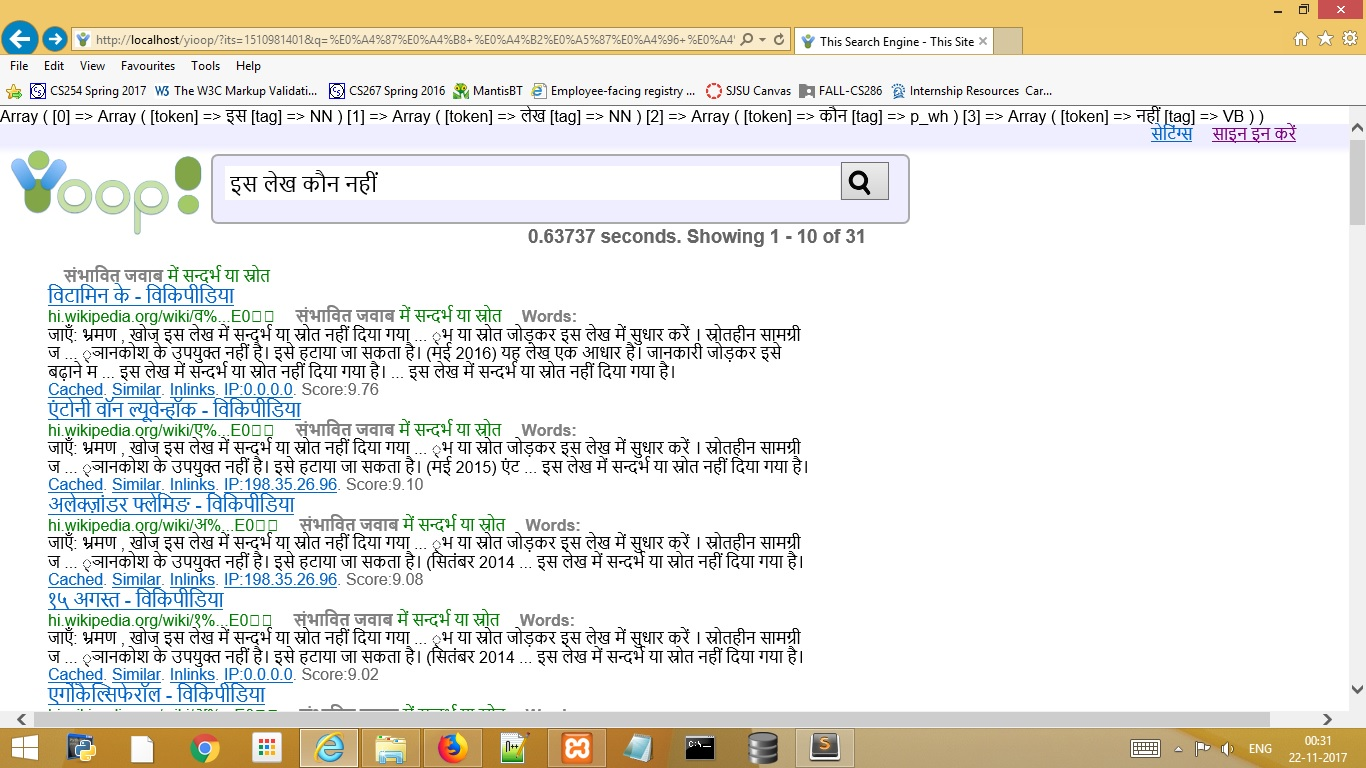
\includegraphics[width=0.8\textwidth]{images/who_question.jpg}
\caption{Who Question.} 
\label{fig:who_question}
\end{figure}

\begin{figure}[htb]
\centering
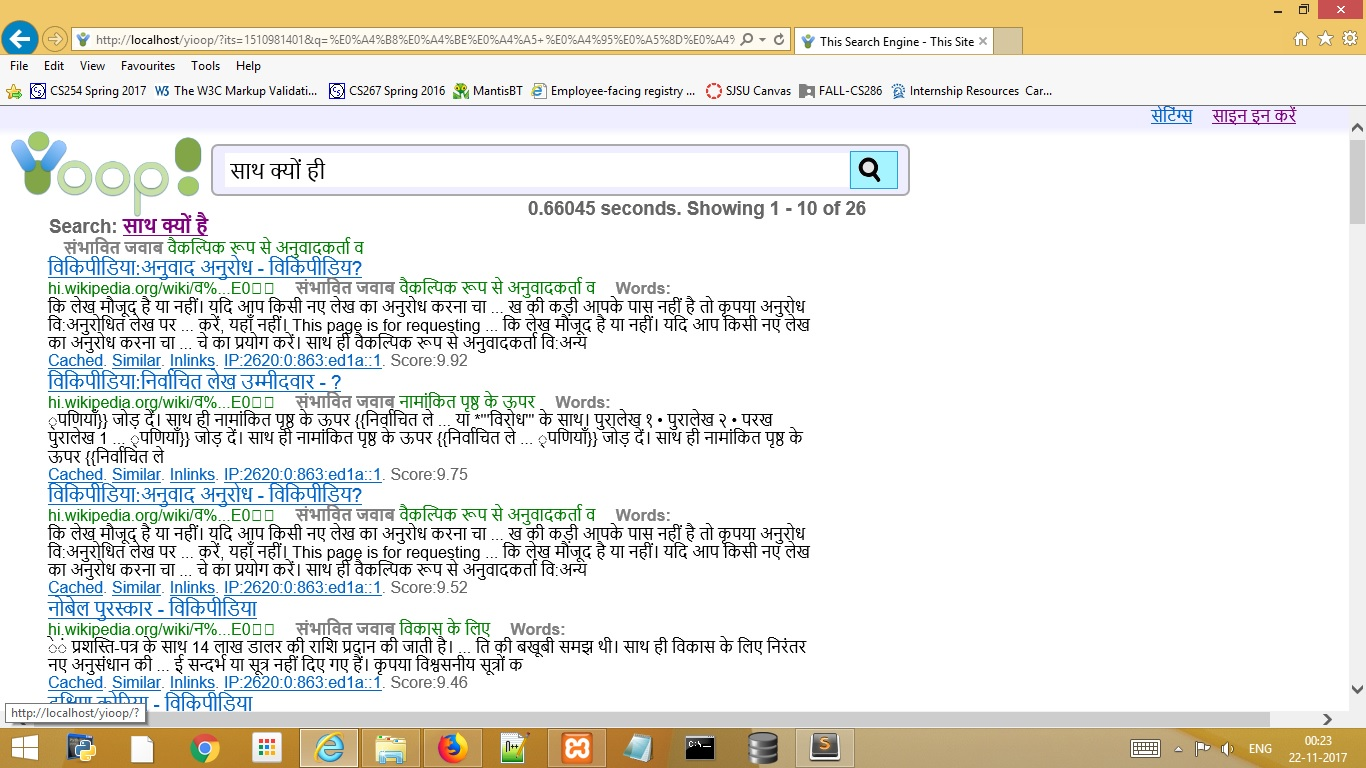
\includegraphics[width=0.8\textwidth]{images/why_question.jpg}
\caption{Why Question.} 
\label{fig:why_question}
\end{figure}

\begin{figure}[htb]
\centering
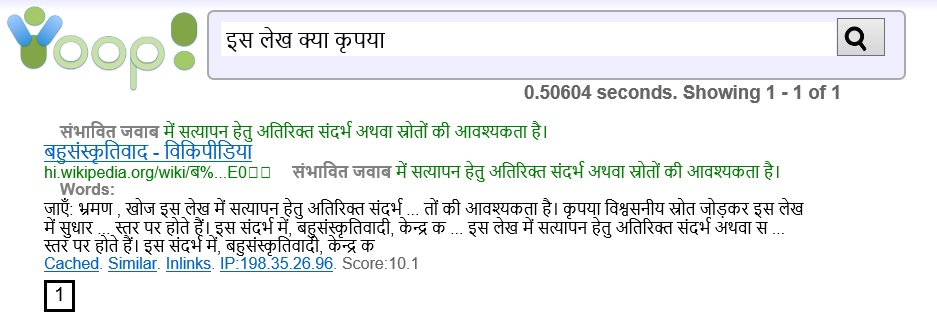
\includegraphics[width=0.8\textwidth]{images/what_question.jpg}
\caption{What Question.} 
\label{fig:what_question}
\end{figure}